\frame[plain]{
    \leftskip-0.4in
    
\begin{tikzpicture}
        \path[fill=white] (0,0) -- (-\paperwidth/2, 0) -- (-\paperwidth/2, \paperheight)
                    --  (0, \paperheight) -- cycle;
        \path[fill=black] (0,0) -- (\paperwidth/2, 0) -- (\paperwidth/2, \paperheight)
                    --  (0, \paperheight) -- cycle;
        \node[black] at (-\paperwidth/4, \paperheight/2) {\xxhuge 0};
        \node[white] at (\paperwidth/4, \paperheight/2) {\xxhuge 1};
    \end{tikzpicture}
}

\frame[plain]{
    \leftskip-0.4in
    \begin{tikzpicture}[remember picture]
        \path[fill=white] (0,0) -- (-\paperwidth/2, 0) -- (-\paperwidth/2, \paperheight)
                    --  (0, \paperheight) -- cycle;
        \path[fill=black] (0,0) -- (\paperwidth/2, 0) -- (\paperwidth/2, \paperheight)
                    --  (0, \paperheight) -- cycle;
        \node[black] at (-\paperwidth/4, \paperheight/3) {\xhuge 0V};
        \node[white] at (\paperwidth/4, \paperheight/3) {\xhuge 3V};
        \node at (0, \paperheight*3/4)
            {{\includegraphics[width=5cm]{processor}}};
        % https://en.wikipedia.org/wiki/File:Cyrix_IBM_CPU_6x86MX_PR200_bottom.jpg
        % Eric Gaba, Wikimedia Commons user Sting
        % CC-BY-SA
        \attributionnode{Image © Eric Gaba, Wikimedia Commons user Sting, CC-BY-SA: \url{https://en.wikipedia.org/wiki/File:Cyrix_IBM_CPU_6x86MX_PR200_bottom.jpg}}
    \end{tikzpicture}
}

\frame[plain]{
    \leftskip-0.4in
    \begin{tikzpicture}
        \path[fill=white] (0,0) -- (-\paperwidth/2, 0) -- (-\paperwidth/2, \paperheight)
                    --  (0, \paperheight) -- cycle;
        \path[fill=black] (0,0) -- (\paperwidth/2, 0) -- (\paperwidth/2, \paperheight)
                    --  (0, \paperheight) -- cycle;
        \node[black] at (-\paperwidth/4, \paperheight/3) {\xhuge };
        \node[white] at (\paperwidth/4, \paperheight/3) {\xhuge \faCircle};
        \node at (0, \paperheight*3/4)
            {{\includegraphics[width=8cm]{punched-tape}}};
        % https://en.wikipedia.org/wiki/File:PaperTapes-5and8Hole.jpg
        % Public Domain
    \end{tikzpicture}
}

\frame[plain]{
    \leftskip-0.4in
    \begin{tikzpicture}
        \path[fill=white] (0,0) -- (-\paperwidth/2, 0) -- (-\paperwidth/2, \paperheight)
                    --  (0, \paperheight) -- cycle;
        \path[fill=black] (0,0) -- (\paperwidth/2, 0) -- (\paperwidth/2, \paperheight)
                    --  (0, \paperheight) -- cycle;
        \node[black] at (-\paperwidth/4, \paperheight/3) {\xhuge S};
        \node[white] at (\paperwidth/4, \paperheight/3) {\xhuge J};
        \node at (0, \paperheight*3/4)
            {{\includegraphics[width=4cm]{floppy-disk}}};
        % https://en.wikipedia.org/wiki/File:Floppy_disk_300_dpi.jpg
        % Public Domain
    \end{tikzpicture}
}

\frame[plain]{
    \leftskip-0.4in
    \begin{tikzpicture}
        \path[fill=white] (0,0) -- (-\paperwidth/2, 0) -- (-\paperwidth/2, \paperheight)
                    --  (0, \paperheight) -- cycle;
        \path[fill=black] (0,0) -- (\paperwidth/2, 0) -- (\paperwidth/2, \paperheight)
                    --  (0, \paperheight) -- cycle;
        \node[black] at (-\paperwidth/4, \paperheight/3) {\xhuge \faEye};
        \node[white] at (\paperwidth/4, \paperheight/3) {\xhuge \faEyeSlash};
        \node at (0, \paperheight*3/4)
            {{\includegraphics[width=4cm]{dvd}}};
        % https://en.wikipedia.org/wiki/File:DVD-Video_bottom-side.jpg
        % Public Domain
    \end{tikzpicture}
}

\frame[plain]{
    \leftskip-0.4in
    
\begin{tikzpicture}
        \path[fill=white] (0,0) -- (-\paperwidth/2, 0) -- (-\paperwidth/2, \paperheight)
                    --  (0, \paperheight) -- cycle;
        \path[fill=black] (0,0) -- (\paperwidth/2, 0) -- (\paperwidth/2, \paperheight)
                    --  (0, \paperheight) -- cycle;
        \node[black] at (-\paperwidth/4, \paperheight/3) {\xhuge \faThumbsDown};
        \node[white] at (\paperwidth/4, \paperheight/3) {\xhuge \faThumbsUp};
        \node at (0, \paperheight*3/4)
            {};
    \end{tikzpicture}
}

\frame[plain]{
    \leftskip-0.4in
    
\begin{tikzpicture}
        \path[fill=white] (0,0) -- (-\paperwidth/2, 0) -- (-\paperwidth/2, \paperheight)
                    --  (0, \paperheight) -- cycle;
        \path[fill=black] (0,0) -- (\paperwidth/2, 0) -- (\paperwidth/2, \paperheight)
                    --  (0, \paperheight) -- cycle;
        \node[black] at (-\paperwidth/4, \paperheight/2) {\xxhuge 0};
        \node[white] at (\paperwidth/4, \paperheight/2) {\xxhuge 1};
    \end{tikzpicture}
}

\frame[plain]{
    \leftskip-0.4in
    \begin{tikzpicture}
        \path[fill=white] (0,0) -- (-\paperwidth/2, 0) -- (-\paperwidth/2, \paperheight)
                    --  (0, \paperheight) -- cycle;
        \path[fill=black] (0,0) -- (\paperwidth/2, 0) -- (\paperwidth/2, \paperheight)
                    --  (0, \paperheight) -- cycle;
        \node[black] at (-\paperwidth/4, \paperheight/3) {\xhuge \faRemove};
        \node[white] at (\paperwidth/4, \paperheight/3) {\xhuge \faCheck};
        \node at (0, \paperheight*5/7) {{\includegraphics[width=2cm]{milk-carton}}};
        % http://www.publicdomainpictures.net/view-image.php?image=118101&picture=milk-carton
        % Public Domain
    \end{tikzpicture}
}

% \frame[plain]{
%     \leftskip-0.4in
%     \begin{tikzpicture}
%         \path[fill=white] (0,0) -- (-\paperwidth/2, 0) -- (-\paperwidth/2, \paperheight)
%                     --  (0, \paperheight) -- cycle;
%         \path[fill=black] (0,0) -- (\paperwidth/2, 0) -- (\paperwidth/2, \paperheight)
%                     --  (0, \paperheight) -- cycle;
%         \node[black] at (-\paperwidth/4, \paperheight/3) {\xhuge \faMars};
%         \node[white] at (\paperwidth/4, \paperheight/3) {\xhuge \faVenus};
%         \node at (0, \paperheight*5/7) {{\includegraphics[width=6cm]{baby}}};
%         % https://en.wikipedia.org/wiki/File:Human-Male-Newborn-Infant-Baby.jpg
%         % Public Domain
%     \end{tikzpicture}
% }

\frame[plain]{
    \leftskip-0.4in
    \begin{tikzpicture}
        \path[fill=white] (0,0) -- (-\paperwidth/2, 0) -- (-\paperwidth/2, \paperheight)
                    --  (0, \paperheight) -- cycle;
        \path[fill=black] (0,0) -- (\paperwidth/2, 0) -- (\paperwidth/2, \paperheight)
                    --  (0, \paperheight) -- cycle;
        \node[black] at (-\paperwidth/4, \paperheight/3) {\xhuge \faLevelUp};
        \node[white] at (\paperwidth/4, \paperheight/3) {\xhuge \faLevelDown};
        \node at (0, \paperheight*5/7) {{\includegraphics[width=3cm]{ladybug}}};
        % http://www.freestockphotos.biz/stockphoto/10710
        % Public Domain
    \end{tikzpicture}
}

\frame[plain]{
    \leftskip-0.4in
    \begin{tikzpicture}[remember picture]
        \path[fill=white] (0,0) -- (-\paperwidth/2, 0) -- (-\paperwidth/2, \paperheight)
                    --  (0, \paperheight) -- cycle;
        \path[fill=black] (0,0) -- (\paperwidth/2, 0) -- (\paperwidth/2, \paperheight)
                    --  (0, \paperheight) -- cycle;
        \node[black] at (-\paperwidth/4, \paperheight/3) {\xhuge \faHeart};
        \node[white] at (\paperwidth/4, \paperheight/3) {\xhuge \faFrownO};
        \node at (0, \paperheight*5/7) {{\includegraphics[width=4cm]{daisy}}};
        % https://commons.wikimedia.org/wiki/File:Leucanthemum_vulgare_qtl1.jpg
        % Wikimedia user Quartl
        % CC-BY-SA 3.0
        \attributionnode{Image © Wikimedia user Quartl, CC-BY-SA: \url{https://commons.wikimedia.org/wiki/File:Leucanthemum_vulgare_qtl1.jpg}}
    \end{tikzpicture}
}

\frame[plain]{
    \leftskip-0.4in
    \begin{tikzpicture}
        \path[fill=white] (0,0) -- (-\paperwidth/2, 0) -- (-\paperwidth/2, \paperheight)
                    --  (0, \paperheight) -- cycle;
        \path[fill=black] (0,0) -- (\paperwidth/2, 0) -- (\paperwidth/2, \paperheight)
                    --  (0, \paperheight) -- cycle;
        \node[black] at (-\paperwidth/4, \paperheight/3) {\xhuge \faSunO};
        \node[white] at (\paperwidth/4, \paperheight/3) {\xhuge \faCloud};
        \node at (0, \paperheight*5/7) {{\includegraphics[width=4cm]{umbrella}}};
        % https://commons.wikimedia.org/wiki/File:Umbrella_opened.svg
        % Public Domain
    \end{tikzpicture}
}

\frame[plain]{
    \leftskip-0.4in
    
\begin{tikzpicture}
        \path[fill=white] (0,0) -- (-\paperwidth/2, 0) -- (-\paperwidth/2, \paperheight)
                    --  (0, \paperheight) -- cycle;
        \path[fill=black] (0,0) -- (\paperwidth/2, 0) -- (\paperwidth/2, \paperheight)
                    --  (0, \paperheight) -- cycle;
        \node[black] at (-\paperwidth/4, \paperheight/2) {\xxhuge 0};
        \node[white] at (\paperwidth/4, \paperheight/2) {\xxhuge 1};
    \end{tikzpicture}
}

\frame {

    {\huge Bude zítra pršet?}
    \pause

    \bigskip

    {\faCaretRight} Ano\\\pause
    {\faCaretRight} Ne\\\pause
    {\faCaretRight} Nevím\\\pause
    {\faCaretRight} S 40\% pravděpodobností\\\pause
    {\faCaretRight} Myslíš v Brně?\\\pause
    {\faCaretRight} Podle jakého modelu?
}

\frame[plain]{

    \bigskip

    {Umíš odpovědět „ano” nebo „ne” na otázku „Bude zítra pršet?”}

    \bigskip

    \pause
    \leftskip-0.4in
    
\begin{tikzpicture}[align=center]
        \path[fill=white] (0,0) -- (-\paperwidth/2, 0) -- (-\paperwidth/2, \paperheight)
                    --  (0, \paperheight) -- cycle;
        \path[fill=black] (0,0) -- (\paperwidth/2, 0) -- (\paperwidth/2, \paperheight)
                    --  (0, \paperheight) -- cycle;
        \node[black,below] at (-\paperwidth/4, \paperheight*7/8) {\faCheck \\ Bude zítra pršet?};
        \pause
        \node[white,below] at (\paperwidth/4, \paperheight*7/8) {\faRemove \\ Aha... \\ A je to tím \\ že to nevíš \\ přesně?};
    \end{tikzpicture}
}

\frame[plain]{

    \bigskip

    Kolik je mi let?

    \bigskip

    \leftskip-0.4in
    
\begin{tikzpicture}[align=center]
        \pause
        \path[fill=white] (0,0) rectangle (-\paperwidth/2, \paperheight);
        \path[fill=black] (0,0) rectangle (\paperwidth/2, \paperheight);
        \node[black,circle,fill=white,draw=black] at (0, \paperheight) {50};
        \pause
        \path[fill=gray] (0,0) rectangle (\paperwidth/2, \paperheight*0.9);
        \node[white] at (\paperwidth/4, \paperheight*0.8) {\faRemove};
        \pause
        \path[fill=white] (-\paperwidth/2,0) rectangle (-\paperwidth/4, \paperheight*0.9);
        \path[fill=black] (-\paperwidth/4,0) rectangle (0, \paperheight*0.9);
        \node[black,circle,fill=white,draw=black] at (-\paperwidth/4, \paperheight*0.9) {25};
        \pause
        \path[fill=gray] (-\paperwidth/2,0) rectangle (-\paperwidth/4, \paperheight*0.8);
        \node[white] at (-\paperwidth*3/8, \paperheight*0.7) {\faRemove};
        \pause
        \path[fill=white] ({\xcoord{25}},0) rectangle ({\xcoord{35}}, \paperheight*0.8);
        \path[fill=black] ({\xcoord{35}},0) rectangle ({\xcoord{50}}, \paperheight*0.8);
        \node[black,circle,fill=white,draw=black] at ({\xcoord{35}}, \paperheight*0.8) {35};
        \pause
        \path[fill=gray] ({\xcoord{35}},0) rectangle ({\xcoord{55}}, \paperheight*0.7);
        \node[white] at ({\xcoord{42.5}}, \paperheight*0.6) {\faRemove};
        \pause
        \path[fill=white] ({\xcoord{25}},0) rectangle ({\xcoord{30}}, \paperheight*0.65);
        \path[fill=black] ({\xcoord{30}},0) rectangle ({\xcoord{35}}, \paperheight*0.65);
        \node[black,circle,fill=white,draw=black] at ({\xcoord{30}}, \paperheight*0.65) {\tiny 30};
        \pause
        \path[fill=gray] ({\xcoord{25}},0) rectangle ({\xcoord{30}}, \paperheight*0.55);
        \pause
        \path[fill=white] ({\xcoord{30}},0) rectangle ({\xcoord{32}}, \paperheight*0.53);
        \path[fill=black] ({\xcoord{32}},0) rectangle ({\xcoord{35}}, \paperheight*0.53);
        \node[black,circle,fill=white,draw=black,inner sep=2pt] at ({\xcoord{32}}, \paperheight*0.53) {\tiny 32}; % 27
        \pause
        \path[fill=gray] ({\xcoord{30}},0) rectangle ({\xcoord{32}}, \paperheight*0.48);
        \pause
        \path[fill=white] ({\xcoord{32}},0) rectangle ({\xcoord{33}}, \paperheight*0.47);
        \path[fill=black] ({\xcoord{33}},0) rectangle ({\xcoord{34}}, \paperheight*0.47);
        \node[black,circle,fill=white,draw=black,inner sep=2pt] at ({\xcoord{33}}, \paperheight*0.47) {\tiny 33}; % 29
        \pause
        \path[fill=gray] ({\xcoord{32}},0) rectangle ({\xcoord{33}}, \paperheight*0.42);
        \pause
        \path[fill=white] ({\xcoord{33}},0) rectangle ({\xcoord{34}}, \paperheight*0.40);
        \path[fill=black] ({\xcoord{34}},0) rectangle ({\xcoord{35}}, \paperheight*0.40);
        \node[black,circle,fill=white,draw=black,inner sep=2pt] at ({\xcoord{34}}, \paperheight*0.40) {\tiny 34}; % 28
        \pause
        \path[fill=gray] ({\xcoord{20}},0) rectangle ({\xcoord{34}}, \paperheight*0.35);
    \end{tikzpicture}
}

\frame[plain]{

    \bigskip

    Myslím si číslo

    \bigskip

    \leftskip-0.4in
    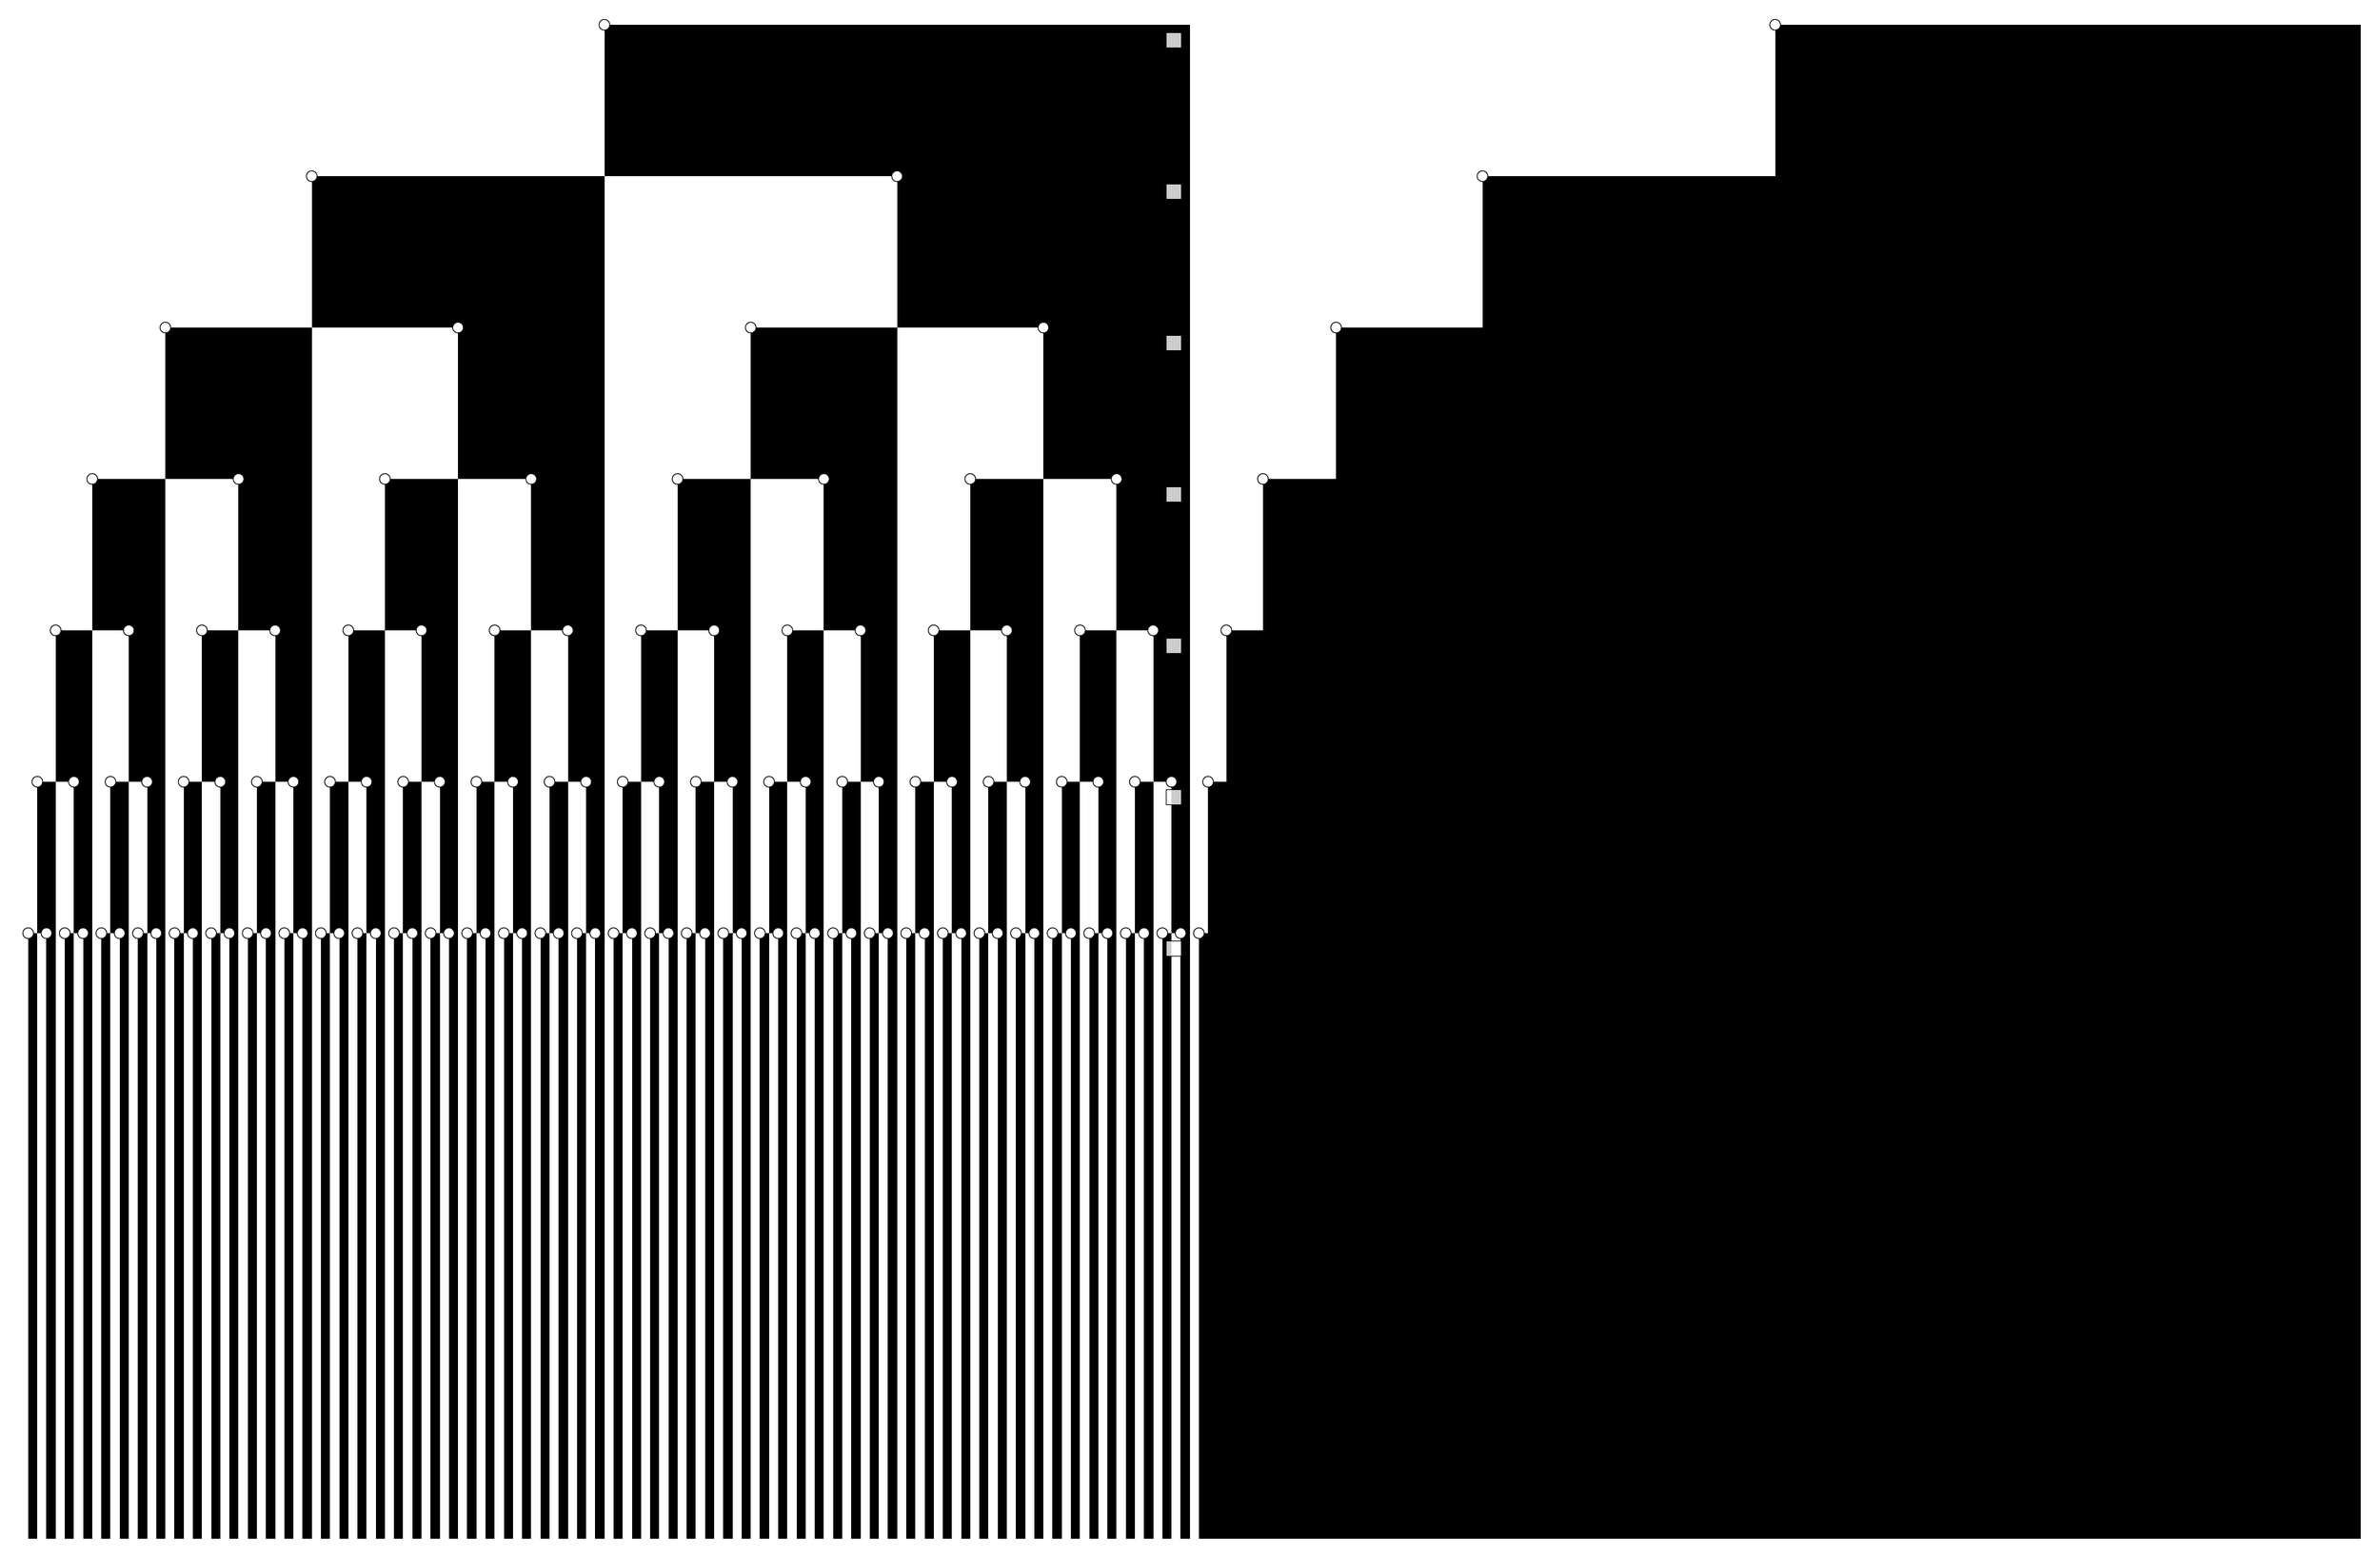
\begin{tikzpicture}[align=center]
        \foreach \m/\y in {1/1, 2/0.9, 4/0.8, 8/0.7,16/0.6,32/0.5,64/0.4} {
            \pause
            \foreach \x in {0,...,\m} {
                \path[fill=white] ({\paperwidth*(-1+(\x+0)/\m)},0) rectangle ({\paperwidth*(-1+(\x+.5)/\m)}, {\paperheight*\y});
                \path[fill=black] ({\paperwidth*(-1+(\x+.5)/\m)},0) rectangle ({\paperwidth*(-1+(\x+1)/\m)}, {\paperheight*\y});
                \node[black,circle,fill=white,draw=black,inner sep=2pt] at ({\paperwidth*(-1+(\x+.5)/\m)}, {\paperheight*\y}) {};
            }
            \tikzmath {integer \mm; \mm = \m*2;}
            \node[below left=4pt,black,rectangle,fill=white,draw=black,inner sep=4pt,fill opacity=0.8] at (0, \paperheight*\y)
                {\tiny \mm};
        }
    \end{tikzpicture}
}

\frame[plain]{

    \bigskip

    Kolik mi je let?

    \bigskip\pause

    \begin{tabular}{rcl}
    64+ ?\pause& \noden{ne}\pause &→ 0-63 \\\pause
    32+ ?& \nodey{ano} &→ 32-63 \\\pause
    48+ ?& \noden{ne} &→ 32-48 \\\pause
    40+ ?& \noden{ne} &→ 32-39 \\\pause
    36+ ?& \noden{ne} &→ 32-35 \\\pause
    34+ ?& \nodey{ano} &→ 34-35 \\\pause
    35 ?& \noden{ne} &→ 34 \\
    \end{tabular}
}

\frame[plain]{

    \bigskip

    Kolik mi je let?

    \bigskip

    \begin{tabular}{rcl}
    \textcolor{white}{64+ ?}& \noden{ne} &\textcolor{white}{→ 0-63} \\
    \textcolor{white}{32+ ?}& \nodey{ano} &\textcolor{white}{→ 32-63} \\
    \textcolor{white}{48+ ?}& \noden{ne} &\textcolor{white}{→ 32-48} \\
    \textcolor{white}{40+ ?}& \noden{ne} &\textcolor{white}{→ 32-39} \\
    \textcolor{white}{36+ ?}& \noden{ne} &\textcolor{white}{→ 32-35} \\
    \textcolor{white}{34+ ?}& \nodey{ano} &\textcolor{white}{→ 34-35} \\
       \textcolor{white}{35 ?}& \noden{ne} &\textcolor{white}{→ 34} \\
    \end{tabular}
}

\frame[plain]{

    \bigskip

    Kolik mi je let?

    \bigskip

    \small
    \noden{0}%
    \nodey{1}%
    \noden{0}%
    \noden{0}%
    \noden{0}%
    \nodey{1}%
    \noden{0}%
}

\frame[plain]{

    \bigskip

    Kolik mi je let?

    \bigskip

    \small
    \begin{tabular}{cr}
     \noden{0} & {\textcolor{ta3aluminium}{+64}} \\
     \nodey{1} & +32 \\
     \noden{0} & {\textcolor{ta3aluminium}{+16}} \\
     \noden{0} & {\textcolor{ta3aluminium}{+8}} \\
     \noden{0} & {\textcolor{ta3aluminium}{+4}} \\
     \nodey{1} & +2 \\
     \noden{0} & {\textcolor{ta3aluminium}{+1}} \\
     \cline{2-2}
     & 34 \\
    \end{tabular}
}


\frame[plain]{

    \bigskip

    Nejen čísla

    \bigskip

    \small
    \begin{tabular}{ccccc}
     00001 & = & 1 & = & A \\
     00010 & = & 2 & = & B \\
     00011 & = & 3 & = & C \\
     00100 & = & 4 & = & D \\
     00101 & = & 5 & = & E \\
     & & ... & & \\
     11010 & = & 26 & = & Z \\
    \end{tabular}
}

\frame[plain]{

    \bigskip

    Nejen čísla

    \bigskip

    \small
    \begin{tabular}{ccccc}
     00101110 & = & 46 & = & . \\
     & & ... & & \\
     01000001 & = & 64 & = & A \\
     01000010 & = & 65 & = & B \\
     01000011 & = & 66 & = & C \\
     & & ... & & \\
     01111011 & = & 193 & = & \{ \\
    \end{tabular}
}

\frame[plain]{
    \leftskip-0.4in
    \begin{tikzpicture}[remember picture]
        \path[fill=white] (0,0) -- (-\paperwidth/2, 0) -- (-\paperwidth/2, \paperheight)
                    --  (0, \paperheight) -- cycle;
        \path[fill=black] (0,0) -- (\paperwidth/2, 0) -- (\paperwidth/2, \paperheight)
                    --  (0, \paperheight) -- cycle;
        \node[black] at (-\paperwidth/4, \paperheight/3) {\xhuge 0V};
        \node[white] at (\paperwidth/4, \paperheight/3) {\xhuge 3V};
        \node at (0, \paperheight*3/4)
            {{\includegraphics[width=5cm]{processor}}};
        % https://en.wikipedia.org/wiki/File:Cyrix_IBM_CPU_6x86MX_PR200_bottom.jpg
        % Eric Gaba, Wikimedia Commons user Sting
        % CC-BY-SA
        \attributionnode{Image © Eric Gaba, Wikimedia Commons user Sting, CC-BY-SA: \url{https://en.wikipedia.org/wiki/File:Cyrix_IBM_CPU_6x86MX_PR200_bottom.jpg}}
    \end{tikzpicture}
}

\frame[t]{
    \begin{tikzpicture}[remember picture,overlay]
    \path[use as bounding box] (0,0);
    % draw image
    \node[inner sep=0] at (current page.center)
        {\includegraphics[width=\paperwidth,height=\paperheight]{atari-800}};
    % https://en.wikipedia.org/wiki/File:Atari_800.jpg
    % Wikimedia user Bilby
    % CC-BY-SA 3.0
    \node[above=5pt,black,fill=white,fill opacity=0.7,text opacity=0.8]
        at(current page.center)
        {8 bitů (1 byte)};
    \node[below=5pt,black,fill=white,fill opacity=0.7,text opacity=0.8]
        at(current page.center)
        {0-255};
    \attributionnode{© Wikimedia user Bilby, CC-BY-SA: \url{https://en.wikipedia.org/wiki/File:Atari_800.jpg}}
    \end{tikzpicture}
}

\frame[t]{
    \begin{tikzpicture}[remember picture,overlay]
    \path[use as bounding box] (0,0);
    % draw image
    \node[inner sep=0] at (current page.center)
        {\includegraphics[width=\paperwidth,height=\paperheight]{amiga}};
    \node[above=5pt,black,fill=white,fill opacity=0.7,text opacity=0.8]
        at(current page.center)
        {16 bitů (2 byty)};
    \node[below=5pt,black,fill=white,fill opacity=0.7,text opacity=0.8]
        at(current page.center)
        {0-65\,535};
    % https://commons.wikimedia.org/wiki/File:Amiga_500_(1987).jpg
    % Dragan at the German language Wikipedia
    % CC-BY-SA 3.0
    \attributionnode{© Dragan at the German language Wikipedia, CC-BY-SA: \url{https://commons.wikimedia.org/wiki/File:Amiga_500_(1987).jpg}}
    \end{tikzpicture}
}

\frame[t]{
    \begin{tikzpicture}[remember picture,overlay]
    \path[use as bounding box] (0,0);
    % draw image
    \node[inner sep=0] at (current page.center)
        {\includegraphics[width=\paperwidth,height=\paperheight]{beige-box}};
    \node[above=5pt,black,fill=white,fill opacity=0.7,text opacity=0.8]
        at(current page.center)
        {32 bitů (4 byty)};
    \node[below=5pt,black,fill=white,fill opacity=0.7,text opacity=0.8]
        at(current page.center)
        {0-4\,294\,967\,295};
    % https://en.wikipedia.org/wiki/File:Beige_Power_Macintosh_G3_Minitower.jpg
    % Public Domain
    \attributionnode{Public Domain image: \url{https://en.wikipedia.org/wiki/File:Beige_Power_Macintosh_G3_Minitower.jpg}}
    \end{tikzpicture}
}

\frame[t]{
    \begin{tikzpicture}[remember picture,overlay]
    \path[use as bounding box] (0,0);
    % draw image
    \node[inner sep=0] at (current page.center)
        {\includegraphics[width=\paperwidth,height=\paperheight]{laptop}};
    \node[above=5pt,black,fill=white,fill opacity=0.7,text opacity=0.8]
        at(current page.center)
        {64 bitů (8 bytů)};
    \node[below=5pt,black,fill=white,fill opacity=0.7,text opacity=0.8]
        at(current page.center)
        {0-18\,446\,744\,073\,709\,551\,615};
    % https://opensource.com/life/15/8/beautiful-super-thin-laptop-makes-fedora-shine
    % Anderson Silva
    % CC BY-SA 4.0
    \attributionnode{© Anderson Silva, CC-BY-SA: \url{https://opensource.com/life/15/8/beautiful-super-thin-laptop-makes-fedora-shine}}
    \end{tikzpicture}
}
